\documentclass[12pt, a4paper]{report}
\usepackage{geometry}

\geometry{
    left=2cm,
    right=2cm,
    top=2cm,
    bottom=2cm,
}

\usepackage[french]{babel}
\usepackage{scrextend}
\usepackage{tcolorbox}
\usepackage{lipsum}
\usepackage{multicol}
\usepackage{amsmath}  % Core AMS math functionality
\usepackage{amssymb}  % Extra math symbols
\usepackage{mathrsfs} % Script fonts (\mathscr)
\usepackage{amssymb}
\usepackage{hyperref}
\usepackage{amsfonts}
\usepackage{amsthm}
\usepackage{csquotes}
\usepackage{hyperref}
\usepackage{needspace}
\usepackage{svg}
\usepackage{listings}
\usepackage{graphicx}

\tcbuselibrary{skins}

\newtcolorbox{mydefinition}[1]{
    colback=blue!5!white,
    colframe=red!75!black,
    fonttitle=\bfseries,
    coltitle=black,
    colbacktitle=red!25!white,
    enhanced,
    attach boxed title to top left={xshift=5mm, yshift=-8.5pt},
    boxed title style={
        boxrule=0.4pt,
        colframe=red!75!black,
        colback=red!25!white,
        rounded corners=10pt,
        arc=5pt,
        boxsep=2pt,
        left=2pt,
        right=2pt,
        top=0pt,
        bottom=1pt,
    },
    title={#1},
    boxrule=1pt,
    rounded corners=3pt,
    arc=3pt,
    boxsep=5pt,
    left=4pt,
    right=4pt,
    top=12pt, % Increased to accommodate the overflowing title
    bottom=5pt,
}

\newtcolorbox{myinfo}[1]{
    colback=blue!5!white,          % Fond du corps de la boîte
    colframe=blue!75!black,        % Bordure de la boîte
    fonttitle=\bfseries,
    coltitle=black,                % Couleur du texte du titre
    colbacktitle=blue!25!white,    % Fond du titre
    enhanced,
    attach boxed title to top left={xshift=5mm, yshift=-8.5pt},
    boxed title style={
        boxrule=0.4pt,
        colframe=blue!75!black,    % Bordure du titre
        colback=blue!25!white,     % Fond du titre
        rounded corners=10pt,
        arc=5pt,
        boxsep=2pt,
        left=2pt,
        right=2pt,
        top=0pt,
        bottom=1pt,
    },
    title={#1},
    boxrule=1pt,
    rounded corners=3pt,
    arc=3pt,
    boxsep=5pt,
    left=4pt,
    right=4pt,
    top=12pt,
    bottom=5pt,
}


\definecolor{keywordcolor}{rgb}{0.13,0.13,1}   % Blue
\definecolor{commentcolor}{rgb}{0.0,0.5,0.0}   % Green
\definecolor{stringcolor}{rgb}{0.58,0,0.82}    % Purple

\lstset{
  language=Java,
  basicstyle=\ttfamily\footnotesize,  % smaller, tighter font
  keywordstyle=\color{keywordcolor}\bfseries,
  commentstyle=\color{commentcolor}\itshape,
  stringstyle=\color{stringcolor},
  showstringspaces=false,
  numbers=left,
  numberstyle=\tiny\color{gray},
  numbersep=5pt,
  frame=single,
  breaklines=true,
  tabsize=2,
  xleftmargin=0pt, % remove extra spacing on left
  xrightmargin=0pt
}


\newcommand{\registeredcompany}[1]{\textit{#1\textsuperscript{\tiny\textregistered}}}

\begin{document}

% HEADER
\noindent
\textbf{Valbonne - Lycée International} \hfill \textbf{FRITES}

\noindent
Le \today{} \hfill Robotique

\par\noindent\rule{\textwidth}{0.5pt}

\vspace{-0.5em} % space between top rule and title

\begin{center}
	\Large Manuel Technique du Robot
\end{center}

\vspace{-0.5em} % space between title and bottom rule

\par\noindent\rule{\textwidth}{0.5pt}

\begin{center}
    % Top Logo
    \vspace*{1cm} % Space from top of page
    \includegraphics[width=0.5\linewidth]{frites_text.png}
    
    % Space between logos
    \vspace{1.5cm}
    
    % Middle Logo
    \includegraphics[width=0.5\linewidth]{FIRST_Tech_challenge_logo.png}
    
    % Space between logos
    \vspace{1.5cm}
    
    % Bottom Logo
    \includegraphics[width=0.5\linewidth]{ftc_decode_1240x860.jpg}
    
    % Space at the bottom
    \vspace*{1cm}
\end{center}

\tableofcontents

\chapter{Introduction}

\section{Objectif}

Notre objectif est de fabriquer le robot le plus performant et fiable pour grimper le plus loin possible dans les classements, mais aussi d'encourager l’esprit d’ingénierie et le travail en équipe. Nous voulons renforcer nos compétences en mécanique, électronique et programmation, appliquer une démarche structurée et collaborative, et développer des solutions innovantes tout en respectant les règles de sécurité et l’éthique de la compétition.

\section{Cahier des charges}

\begin{mydefinition}{Cahier des charges}
Un cahier des charges est un document qui décrit l’ensemble des besoins, contraintes et spécifications techniques qu’un produit ou un système doit respecter. Il sert de référence tout au long de la conception et de la réalisation.
\end{mydefinition}

\subsection{Cahier des charges officiel \registeredcompany{FIRST}}
Un cahier des charges complet est fourni par \registeredcompany{FIRST}. Celui-ci décrit toutes les contraintes précises du robot, ainsi que les caractéristiques du terrain et les règles à respecter avant, pendant et après les matchs.

Veuillez retrouver celui-ci à l’adresse suivante : \url{https://ftc-resources.firstinspires.org/ftc/game/manual}.

\subsection{Résumé du cahier des charges, points importants à retenir et contraintes personnelles}

\subsubsection{Éligibilité et inspection des robots}

Le robot doit tenir dans un volume de 18 pouces x 18 pouces x 18 pouces (soit 45,7 cm x 45,7 cm x 45,7 cm). Pour cette saison, les robots n'ont pas le droit de s'étendre au-delà de ces dimensions, sauf pour la fin du match (\textit{l'\enquote{endgame}}, les dernières 20 secondes du match).

\begin{mydefinition}{Taille maximale du robot}
La taille maximale initiale d’un robot pour cette saison est de 45,7 cm x 45,7 cm x 45,7 cm. Il ne peut pas dépasser ces dimensions sauf durant l'\textit{endgame}.
\end{mydefinition}

L'équipe des FRITES a décidé d'utiliser principalement des composants \registeredcompany{GoBilda}. Il convient donc d'utiliser des pièces \registeredcompany{GoBilda} autant que possible et d'éviter les autres marques afin de prévenir les problèmes d'incompatibilité. Cependant, certaines exceptions existent, comme par exemple les \textit{\enquote{Control Hubs}}, qui sont principalement fournis par \registeredcompany{REV}.

En respectant ces critères, l'équipe s'assure que le robot sera conforme aux règles de la compétition et pourra passer l'inspection sans difficultés, tout en minimisant les risques d'incompatibilités entre composants.

\subsubsection{Dimensions principales à retenir}

Voici une liste (non exhaustive) des contraintes de dimensions à respecter pour les matchs:
\begin{itemize}
    \item Le robot doit tenir dans un volume de 18 pouces x 18 pouces x 18 pouces (soit 45,7 cm x 45,7 cm x 45,7 cm).
    \item Terrain: 144 pouces par 144 pouces (soit 365,75 cm by 365,75 cm)
    \item \enquote{Artifact}: 5 pouces de diamètre (soit 12,70 cm)
\end{itemize}

\subsubsection{Caractéristiques spécifiques à la saison}

Cette saison du \textit{FIRST\textsuperscript{\tiny\textregistered} Tech Challenge}, intitulée \textbf{DECODE\texttrademark}, se concentre sur un jeu dynamique où deux alliances de deux robots s'affrontent pour marquer des \textit{artéfacts} (objets violets et verts) dans un but, construire des \textit{motifs} sur une rampe selon un schéma aléatoire affiché sur un obélisque, et revenir à leur base avant la fin du match. Le match se déroule en deux phases : \textbf{30 secondes en mode autonome}, où les robots doivent décoder le motif et commencer à marquer, suivies de \textbf{2 minutes en mode télécommandé}, où les pilotes optimisent le score.

Les équipes sont évaluées sur leur \textbf{performance technique}, leur \textbf{documentation} (portfolio, processus de conception), et leur \textbf{engagement communautaire}. Les récompenses, comme l'\textit{Inspire Award} ou le \textit{Think Award}, mettent en avant l'excellence globale, la créativité, et l'impact social. Les robots doivent respecter des contraintes strictes, notamment une \textbf{taille initiale maximale de 45,7 cm x 45,7 cm x 45,7 cm}, tout en restant stables et sûrs.

Cette saison encourage l'\textbf{innovation}, la \textbf{stratégie d'alliance}, et la \textbf{collaboration} entre équipes, dans un esprit de compétition équilibré par l'entraide et le respect des valeurs \textit{FIRST}.

\section{Résumé}
\begin{itemize}
\item Construire un robot performant pour le \textit{FTC} et développer les compétences de l’équipe (mécanique, électronique, code).
\item Respecter les contraintes officielles : robot limité à \textbf{18" x 18" x 18"}, terrain de \textbf{144" x 144"}, artéfacts de \textbf{Ø 5"}.
\item Suivre le cahier des charges \registeredcompany{FIRST} + contraintes internes (usage majoritaire de pièces \registeredcompany{GoBilda}).
\item Prendre en compte les phases du match : \textbf{30 s} autonome + \textbf{120 s} téléopéré.
\item Réaliser les objectifs du jeu DECODE™ : dépôt d’artéfacts, construction de motifs, retour à la base.
\item Répondre aux critères d’évaluation : performance du robot, conformité, documentation, engagement de l’équipe.
\end{itemize}

\chapter{Conception Mécanique}

La conception mécanique constitue la base du robot et détermine sa robustesse, sa stabilité et sa capacité à accomplir les tâches prévues sur le terrain.

Ce chapitre abordera tous ces aspects afin de présenter une approche structurée et cohérente, garantissant un robot fiable, performant et conforme aux règles de la compétition.

\section{Châssis et structure}

\begin{mydefinition}{Châssis}
Le châssis constitue la structure principale du robot, assurant la rigidité nécessaire pour supporter les systèmes de locomotion, de manipulation et d'alimentation, tout en respectant les contraintes de dimensions et de poids imposées par la compétition.
\end{mydefinition}

\subsection{Plateforme de base}

\begin{figure}[h]
    \centering
    
\includegraphics[width=0.4\linewidth]{ROBOT-BOTTOM.pdf}
    \caption{Plateforme de base du robot simplifiée}
    \label{fig:robot-bottom}
\end{figure}

La plateforme de base est un élément essentiel du robot, puisqu'elle supporte l'ensemble des systèmes, y compris les roues et tous les mécanismes supérieurs.  

Notre base, ainsi que la majorité des autres composants, est fabriquée à partir de profilés métalliques \registeredcompany{GoBilda}, choisis pour leur rigidité, leur légèreté et leur modularité, ce qui facilite l'assemblage et la maintenance.

Après l'assemblage de ce module essentiel, on peut y rajouter les roues. Nous avons choisi d'utiliser des roues \textit{GripForce\textsuperscript{\texttrademark}} (SKU \href{https://www.gobilda.com/gripforce-mecanum-wheel-set-o104mm-40a-durometer-rollers/}{3625-0202-0104}) par \registeredcompany{GoBilda}, qui permettent au robot de se déplacer latéralement en faisant tourner les roues de chaque côté en sens opposés.

De plus, nous utlisions des moteurs (SKU \href{https://www.gobilda.com/5203-series-yellow-jacket-planetary-gear-motor-19-2-1-ratio-24mm-length-8mm-rex-shaft-312-rpm-3-3-5v-encoder/}{5203-2402-0019}) assemblés perpendiculairement pour alimenter les quatres roues en utilisant le moins de place possible. Voici à quoi cela ressemble:

\begin{figure}[h]
    \centering
    \includegraphics[width=0.5\linewidth]{ROBOT-BOTTOM-WHEELS.png}
    \caption{Plateforme de base du robot après installation des roues et moteurs}
    \label{fig:robot-bottom}
\end{figure}

\subsection{Entrée (\enquote{intake})}

L'\enquote{intake} permet, comme son nom l'indique, de faire entrer des \textit{artifacts} dans le module de stockage et de triage, appelé le \enquote{buffer}. Il a été conçu pour ramasser les \textit{artifacts} directement au sol et les acheminer rapidement dans le buffer.

Il est composé de deux axes horizontaux :  
\begin{itemize}
    \item un axe avec des roues \textit{Gecko}\textsuperscript{\texttrademark} \registeredcompany{GoBilda} de 32 mm (SKU \href{https://www.gobilda.com/gripforce-gecko-wheel-8mm-rex-bore-32mm-diameter/}{3613-4008-0032}) ;  
    \item un axe avec des roues d'intake de 72 mm (SKU \href{https://www.gobilda.com/3615-series-boot-wheel-8mm-rex-bore-72mm-diameter-30a-durometer/}{3615-4008-0072}) reliées à un moteur 312 rpm via une chaîne.
\end{itemize}

\begin{myinfo}{Problèmes connus}
Il est presque impossible de faire entrer plusieurs \textit{artifacts} de manière successive et rapide, en raison des limites de vitesse du servo sélecteur, qui assure le tri des \textit{artifacts}.

Il est donc recommandé d’éviter de ramasser les \textit{artifacts} trop rapidement afin de prévenir leur éjection accidentelle, le blocage de l'intake, ou même la détérioration d’un servo.
\end{myinfo}

\begin{figure}[h]
    \centering
    \includegraphics[width=0.17\linewidth]{ROBOT-INTAKE.png}
    \caption{Intake du robot, vue de côté}
    \label{fig:robot-intake}
\end{figure}

\needspace{8\baselineskip}
\subsection{\enquote{Buffer} et lanceur}

Le buffer permet de temporairement bloquer un ou plusieurs \textit{artifacts} dans le robot. Cela est généralement réalisé dans les cas suivants:
\begin{itemize}
    \item Attendre que le robot se positionne vers le but;
    \item Attendre que la roue libre du lanceur (\enquote{flywheel}) accélère ou ralentisse pour atteindre sa vitesse cible;
    \item Attendre la confirmation du driver pour tirer;
    \item Attendre la confirmation de l'ordinateur pour assurer un tir réussi.
\end{itemize}

Une fois la décision prise, un de deux servos s'activera, qui poussera l'artifact dans le lanceur.

\begin{myinfo}{Problèmes connus}
La pièce qui propulse les \textit{artifacts} dans le lanceur peut parfois se bloquer. La cause exacte n’est pas encore déterminée, mais cela pourrait être lié aux trous présents dans les \textit{artifacts}.

En cas de blocage, il suffit généralement d’arrêter puis de redémarrer le servo une ou plusieurs fois pour que l’\textit{artifact} soit correctement éjecté.
\end{myinfo}

Le lanceur permet, comme son nom l'indique, de lancer les \textit{artifacts} le plus précisément possible dans le but. Il consiste d'une flywheel accélérée par deux moteurs 6000 rpm (SKU \href{https://www.gobilda.com/5203-series-yellow-jacket-motor-1-1-ratio-24mm-length-8mm-rex-shaft-6000-rpm-3-3-5v-encoder/}{5203-2402-0001}) et d'une rampe.

\begin{figure}[h]
    \centering
    \includegraphics[width=0.4\linewidth]{ROBOT-LAUNCHER.png}
    \caption{Lanceur du robot}
    \label{fig:robot-intake}
\end{figure}

\section{Diagrammes et CAD}

Des diagrammes pour le robot sont disponibles. Ceux-ci sont distribués au format .easm, qui peut être lu par SOLIDWORKS ou eDrawings.

\begin{mydefinition}{Comment obtenir ces logiciels?}
    SOLIDWORKS est une application payante qui permet de modifier le fichier, il n'est donc pas recommandé de l'utiliser uniquement pour la lecture de ce fichier.

    En parallèle, eDrawings Viewer et un logiciel de la même entreprise qui permet de lire ce fichier et obtenir les références de toutes les pièces. Il est recommandé d'utiliser la version Windows pour avoir plus de performance.
    
    Téléchargez le ici: \url{https://www.edrawingsviewer.com/download-edrawings}.
\end{mydefinition}

\begin{figure}[h]
    \centering
    \includegraphics[width=1\linewidth]{ROBOT-EDRAWINGS.png}
    \caption{Robot prévisualisé dans le lecteur eDrawings}
    \label{fig:robot-intake}
\end{figure}


\chapter{Système Électrique}

\section{Architecture électrique}

\begin{figure}[htbp]
  \centering
\includesvg[width=1\linewidth]{ROBOT-CH-DIAGRAM.svg}
\end{figure}

\begin{mydefinition}{Note sur le schéma électrique}
Ce schéma représente l’architecture électrique générale du robot, mais il n’est pas obligatoire de le suivre exactement. L’important est que tous les composants soient correctement connectés et que chaque élément soit correctement déclaré et référencé dans le \textit{Driver Station}.
\end{mydefinition}


\chapter{Programmation}

\section{Environnement et outils}

\subsection{Outils nécessaires et recommandés}

La base de code du robot est écrite en Java, avec l'utilisation des bibliothèques officelles \registeredcompany{First}, qui permettent une interface facilitée avec les différents composants du robot. Le FTC SDK peut être retrouvé ici: \url{https://github.com/FIRST-Tech-Challenge/FtcRobotController}.

\begin{mydefinition}{FTC SDK}
    Le SDK officel et open source de \registeredcompany{First} est disponible ici: \url{https://github.com/FIRST-Tech-Challenge/FtcRobotController}. 
\end{mydefinition}

L'équipe a recyclé le code de l'année dernière pour gagner du temps et éviter de re-tomber sur des bugs des années précédentes. C'est pour cela qu'il est \textbf{nécessaire d'utiliser Java 21} pour compiler le code.

De plus, il est fortement recommandé d'utiliser un IDE pour pouvoir compiler et publier le code facilement. Nous recommandons l'utilisation de \textbf{Android Studio}, car il contient de nombreuses fonctionnalités avancées permettant d’accélérer le développement, mais permet aussi de compiler et publier son code facilement. Pour cela, \textbf{le reste de la documentation assumera l'utilisation d'Android Studio}.

\begin{myinfo}{Résumé des outils nécessaires}
    Voici les outils nécessaires pour le développement et la programmation:
    \begin{itemize}
        \item Java Development Kit (JDK) \textbf{21}
        \item Android Studio
    \end{itemize}
    L'utilisation de ces éléments avec les bonnes versions est essentiel. Le reste de la documentation assumera leur bonne utilisation.
\end{myinfo}

\subsection{Préparation de l'environnement}

Comme indiqué précédemment, \textbf{il faut obligatoirement avoir JDK 21 et Android Studio}. Il faut aussi avoir un access au dépot git sur Gitlab (Pour vérifier: \url{https://gitlab.com/ftc-civ/frites/2026}).

\subsubsection{Téléchargement du code source}

Ceci peut être réalisé de plusieures manières. La plus simple est d'utiliser la fonctionnalité git dans Android Studio, qui téléchargera et préparera automatiquement le projet.

\begin{figure}[h]
    \centering
    \includegraphics[width=0.8\linewidth]{CLONE.png}
    \caption{Capture d'écran de la fenêtre clone dans Android Studio}
    \label{fig:placeholder}
\end{figure}

Il est aussi possible d'utiliser directement l'outil de CLI \verb|git|:

\begin{verbatim}
git clone git@gitlab.com:ftc-civ/frites/2026.git
\end{verbatim}

\subsubsection{Initialization}

Dans des conditions normales, Android Studio prépare automatiquement le projet avec Gradle, qui téléchargera toutes les bibliothèques automatiquement. Dans ce cas, cette étape n'est pas nécessaire.

Sinon, il faut cliquer sur le bouton \enquote{Download sources} dans l'onglet Gradle.

\begin{figure}[h]
    \centering
    \includegraphics[width=0.5\linewidth]{SETUP-GRADLE.png}
    \caption{Menu Gradle dans Android Studio}
    \label{fig:placeholder}
\end{figure}

\subsubsection{Compilation et publication}

Une fois des modifications éffectuées, il convient de compiler le code. Pour cela, il faut appuyer sur l'icone \enquote{build} (représentée par un marteau) pour compiler le code.

Pour publier le code il faut premièrement connecter le control hub du robot à son ordinateur. Cela peut se faire de deux façons :
\begin{itemize}
    \item \textbf{Par USB} (uniquement sous Windows) en branchant directement le control hub à l’ordinateur.
    \item \textbf{Par Wi-Fi}, méthode généralement plus simple et plus fiable, en se connectant au réseau Wi-Fi du control hub, puis en utilisant la commande \texttt{adb connect} sur l’adresse IP du routeur, en général \texttt{192.168.43.1}. Une fois la connexion établie, il est alors possible de publier le code vers le robot via Android Studio.
\end{itemize}

\begin{figure}[h]
    \centering
    \includegraphics[width=0.8\linewidth]{BUILD-CODE.png}
    \caption{Capture d'écran des boutons \enquote{Build} et \enquote{Start}}
    \label{fig:placeholder}
\end{figure}

Il suffit ensuite de cliquer sur le bouton \enquote{Start} dans Android Studio, après s’être assuré que la bonne cible (\enquote{target}) est sélectionnée et que le robot est correctement connecté. Le transfert peut parfois prendre une à deux minutes avant d’aboutir.

\section{Architecture logicielle}

\subsection{Conventions internes}

Les conventions internes définissent les règles à suivre pour garantir un code lisible, cohérent et maintenable. Elles sont regroupées par thèmes pour faciliter la lecture.

\subsubsection*{Nommage des éléments}
\begin{itemize}
    \item \textbf{Classes :} \texttt{PascalCase} (ex : \texttt{DriveSubsystem}, \texttt{IntakeMotor})
    \item \textbf{Méthodes / fonctions :} \texttt{camelCase} (ex : \texttt{setPower()}, \texttt{runIntake()})
    \item \textbf{Variables :} \texttt{camelCase} pour les variables locales, \texttt{UPPER\_SNAKE\_CASE} pour les constantes
    \item \textbf{Packages / dossiers :} minuscules, sans espaces (ex : \texttt{subsystems}, \texttt{opmodes})
    \item \textbf{Boutons de gamepad :} noms explicites (ex : \texttt{buttonA}, \texttt{leftTrigger})
\end{itemize}

\begin{mydefinition}{À retenir}
Un bon nommage facilite la lecture et la maintenance du code, surtout lorsque plusieurs développeurs travaillent sur le même projet. Il est toujours mieux d'écrire des noms d'objets très longs plutôt que quelque chose d'ambigu.
\end{mydefinition}

\needspace{\7\baselineskip}
\subsubsection*{Organisation des fichiers}
\begin{itemize}
    \item Une classe par fichier, nom du fichier = nom de la classe
    \item Ordre recommandé dans le fichier :
    \begin{enumerate}
        \item Déclarations des constantes
        \item Variables d’instance
        \item Constructeur / initialisation
        \item Méthodes publiques
        \item Méthodes privées / utilitaires
    \end{enumerate}
\end{itemize}

\subsubsection*{Documentation et commentaires}
\begin{itemize}
    \item Chaque sous-système et méthode publique doit être commenté
    \item Expliquer le rôle des paramètres et des valeurs retournées
    \item Utiliser \texttt{TODO} et \texttt{FIXME} pour signaler le code en développement
\end{itemize}

\subsubsection*{Bonnes pratiques}
\begin{itemize}
    \item Initialiser le matériel dans \texttt{init()} ou dans le constructeur de la classe Hardware
    \item Respecter les limites physiques et logicielles des moteurs et servos
    \item Préférer des méthodes courtes et claires plutôt que longues et complexes
    \item Tester chaque sous-système indépendamment avant de l’intégrer aux OpModes
\end{itemize}

\begin{myinfo}{Astuce pratique}
Avant chaque commit Git, vérifier que le code respecte les conventions de nommage et de formatage.
\end{myinfo}

\subsubsection*{Formatage et style}
\begin{itemize}
    \item Indentation : 4 espaces
    \item Accolades : sur la même ligne pour les méthodes et les blocs
    \item Espaces autour des opérateurs
    \item Longueur de ligne recommandée : maximum 120 caractères
\end{itemize}

\subsection{Structure générale}

Le projet est organisé de manière modulaire pour séparer clairement les responsabilités et faciliter la maintenance. Sa structure est basée sur le FTC SDK. Chaque dossier a un rôle précis, décrit ci-dessous.

\subsubsection*{Racine du projet}
\begin{itemize}
    \item \texttt{build.gradle}, \texttt{settings.gradle}, \texttt{gradle.properties} : fichiers de configuration du projet et de Gradle
    \item \texttt{gradlew}, \texttt{gradlew.bat} : scripts pour exécuter Gradle localement
    \item \texttt{libs} : bibliothèques et keystore pour le déploiement sur Android
    \item \texttt{images} : ressources graphiques pour le manuel ou l'interface
\end{itemize}

\needspace{10\baselineskip}
\subsubsection*{FtcRobotController}

\begin{mydefinition}{FtcRobotController}
La librairie officielle de \registeredcompany{First} qui contient l’application Android du robot, les OpModes d’exemple et les classes internes nécessaires à l’exécution du robot sur le téléphone.  
C’est la base sur laquelle tout le code spécifique de l’équipe s’appuie.
\end{mydefinition}

Contient l’application principale du robot. Il ne doit pas être modifié.  
\begin{itemize}
    \item \texttt{src/main/java/org/firstinspires/ftc/robotcontroller} : code source principal, incluant :
    \begin{itemize}
        \item \texttt{external/samples} : exemples d’OpModes et de gestion du hardware
        \item \texttt{external/externalhardware} : classes de configuration de hardware personnalisées
        \item \texttt{internal} : classes internes pour l’application, comme l’enregistrement des OpModes et les activités Android
    \end{itemize}
    \item \texttt{src/main/res} : ressources Android (layouts, drawables, menus, sons)
\end{itemize}

\subsubsection*{TeamCode}
C’est ici que se trouve le code spécifique à l’équipe.  
\begin{itemize}
    \item \texttt{src/main/java/core} : code principal du robot, structuré en sous-dossiers :
    \begin{itemize}
        \item \texttt{localization} : gestion de la position du robot (Odometry, Limelight)
        \item \texttt{logic} : actions et gestion du terrain
        \item \texttt{math} : classes utilitaires pour la géométrie et les unités
        \item \texttt{modules} : sous-systèmes du robot (Intake, Cannon, GamepadController, etc.)
        \item \texttt{opmodes} : OpModes autonomes et téléop, avec versions par équipe/couleur
    \end{itemize}

    \begin{mydefinition}{Roadrunner}
    Une librairie de trajectoire et de cinématique pour robots FTC. Elle fournit des localisateurs (localizers), des calculs de trajectoire et des abstractions pour différents types de châssis (tank, mecanum, etc.).  
    Elle est utilisée pour la navigation précise et l’exécution des trajectoires autonomes.
    \end{mydefinition}

        \begin{itemize}
        \item \texttt{roadrunner} : code de trajectoire et localisateurs
        \item \texttt{debug} : outils de test et d’inspection
        \item \texttt{messages} : classes pour échanger des données entre modules
    \end{itemize}
    \item \texttt{src/main/assets/trajectory} : fichiers de trajectoire pour les OpModes autonomes
    \item \texttt{src/main/res} : ressources additionnelles pour TeamCode
\end{itemize}

\subsubsection*{Modules supplémentaires}
\begin{itemize}
    \item \texttt{Inertia} : librairie interne pour la sérialisation, le stockage et le replay des données
    \item \texttt{MeepMeep} : simulation et visualisation des trajectoires (hors robot réel)
\end{itemize}

\begin{myinfo}{Résumé}
Cette organisation permet de séparer clairement :
\begin{itemize}
    \item le code de base du SDK (\texttt{FtcRobotController}) ;
    \item le code spécifique à l’équipe (\texttt{TeamCode}) ;
    \item les bibliothèques et outils de simulation (\texttt{Inertia}, \texttt{MeepMeep}) ;
    \item et les ressources (assets, sons, images, configurations Android).
\end{itemize}
Elle facilite la réutilisation de code et le débogage.
\end{myinfo}

\subsection{Systèmes de coordonnées}

\needspace{9\baselineskip}
\subsubsection*{Préface}

Veuillez lire attentivement cette section afin d'éviter des bugs subtils liés à des systèmes de coordonnées non correspondants.

La base de code utilise plusieurs systèmes de coordonnées avec différentes directions d'axes,
origines et sens de rotation. Ces différences sont imposées par des bibliothèques tierces
(par exemple, le SDK FTC, Road Runner, les pilotes matériels) et ne peuvent pas être modifiées.

Mélanger des systèmes de coordonnées sans conversion appropriée entraîne des bogues difficiles à déboguer et à comprendre, compromettant tout le système de navigation. Ce document vise à clarifier les systèmes de coordonnées et à établir des directives strictes pour éviter tout problème.

\subsubsection*{Directives}

Pour éviter toute confusion et bugs, nous adoptons les directives suivantes. Consultez la section \ref{coordinate-systems} pour les détails sur chaque système de coordonnées.

\begin{itemize}
    \item Toute la logique interne doit utiliser uniquement le \textbf{système de coordonnées standard}.
    \item Les systèmes de coordonnées spécifiques aux bibliothèques sont autorisés \textbf{uniquement aux frontières}, c'est-à-dire lors de l'interface en entrée ou en sortie avec une bibliothèque. Ils doivent être convertis en système de coordonnées standard avant toute utilisation ultérieure. Toute violation de cette règle doit être clairement documentée.
    \item \textbf{Centraliser} toutes les conversions de systèmes de coordonnées dans des fonctions utilitaires définies dans les classes \texttt{Pose2D} (ou classes connexes).
    \item Les systèmes de coordonnées des nouvelles bibliothèques positionnelles doivent être \textbf{documentés} dans ce fichier.
\end{itemize}

\subsubsection*{Systèmes de coordonnées}
\label{coordinate-systems}

\paragraph{Système de coordonnées standard}

\begin{itemize}
    \item Origine : Centre du terrain
    \item Axe X : X positif pointant vers le côté du public
    \item Axe Y : Y positif pointant vers le côté de l'alliance bleue
    \item Rotation zéro : Direction de l'axe +X
    \item Sens de rotation : Rotation positive dans le sens anti-horaire
    \item Unités : Toutes unités, utilisées via des classes auto-convertibles (par ex. \texttt{Pose2D}, \texttt{Distance}, etc.)
\end{itemize}

\needspace{17\baselineskip}
\paragraph{Système de coordonnées FTC}

\begin{itemize}
    \item Origine : Centre du terrain
    \item Axe X : X positif pointant vers le côté du public
    \item Axe Y : Y positif pointant vers le côté de l'alliance bleue
    \item Rotation zéro : Direction de l'axe +X
    \item Sens de rotation : Rotation positive dans le sens anti-horaire
    \item Unités : Pouces, degrés. Elles sont généralement auto-converties lors de l'accès.
\end{itemize}

\begin{figure}[h]
    \centering
    \includegraphics[width=0.8\linewidth]{DECODE-FIELD.png}
    \caption{Illustration du systeme FTC}
    \label{fig:placeholder}
\end{figure}

\needspace{1\baselineskip}
\paragraph{Système de coordonnées Road Runner}

Relatif au robot

\begin{itemize}
    \item Origine : Centre du robot
    \item Axe X : X positif pointant vers la droite du robot
    \item Axe Y : Y positif pointant vers l'avant du robot
    \item Rotation zéro : Direction de l'axe +Y
    \item Sens de rotation : Rotation positive dans le sens anti-horaire
    \item Unités : Radians. Il n'impose pas d'unité de distance, nous utilisons donc des classes auto-convertibles (par ex. \texttt{Pose2D}, \texttt{Distance}, etc.)
\end{itemize}

\paragraph{Système de coordonnées du pilote Gobilda Pinpoint}

Peut fonctionner en mode absolu ou relatif.

\subparagraph{Mode absolu}

Le mode absolu utilise le système de coordonnées FTC.

\subparagraph{Mode relatif}

Le mode relatif est défini comme suit :

\begin{itemize}
    \item Origine : Centre du robot
    \item Axe X : X positif pointant vers l'avant du robot
    \item Axe Y : Y positif pointant vers la gauche du robot
    \item Sens de rotation : Rotation positive dans le sens anti-horaire
    \item Unités : Pouces, degrés. Elles sont généralement auto-converties lors de l'accès.
\end{itemize}


\section{Tests et débogage}

Avant de lancer un OpMode complet, il est important de tester le robot en conditions réelles pour s'assurer que chaque sous-système fonctionne correctement. Cette section présente les méthodes de test et les outils de débogage recommandés pour le développement et la compétition. Les tests peuvent se faire en mode TeleOp, avec des OpModes autonomes simplifiés, ou à l'aide d'outils spécifiques pour vérifier les moteurs, servos et capteurs.

\needspace{10\baselineskip}
\subsection{Modes TeleOp}


Les \textbf{modes TeleOp} (ou téléopération) sont des programmes permettant de contrôler le robot manuellement via les gamepads. Ces modes sont utilisés pour tester le robot, ajuster les mécaniques en conditions réelles et pour la partie du match où le pilote prend le contrôle.

\begin{mydefinition}{TeleOp}
Un \textit{TeleOp} est un \texttt{OpMode} qui lit les entrées des gamepads et agit en conséquence sur les moteurs, servos et autres composants. Contrairement aux OpModes autonomes, il ne suit pas de trajectoire prédéfinie.
\end{mydefinition}

\needspace{15\baselineskip}
\subsubsection*{Écrire un TeleOp simple}

Voici un exemple minimaliste d’OpMode TeleOp pour contrôler un moteur à l’aide du joystick gauche :

\begin{lstlisting}[language=Java]
package core.opmodes;

import com.qualcomm.robotcore.eventloop.opmode.LinearOpMode;
import com.qualcomm.robotcore.hardware.DcMotor;

@com.qualcomm.robotcore.eventloop.opmode.TeleOp(name="SimpleTeleOp")
public class SimpleTeleOp extends LinearOpMode {
    private DcMotor leftMotor;

    @Override
    public void runOpMode() {
        leftMotor = hardwareMap.get(DcMotor.class, "left_motor");
        waitForStart();

        while (opModeIsActive()) {
            double power = -gamepad1.left_stick_y;
            leftMotor.setPower(power);
        }
    }
}
\end{lstlisting}

\begin{myinfo}{À retenir}
\begin{itemize}
    \item Toujours initialiser le hardware avant \texttt{waitForStart()}.
    \item Utiliser \texttt{opModeIsActive()} pour que la boucle se termine si l'OpMode est stoppé.
    \item Lire les valeurs du gamepad et les convertir en puissance ou commandes pour les moteurs/servos.
\end{itemize}
\end{myinfo}

\subsubsection*{OpModes TeleOp disponibles}

Le robot dispose de plusieurs OpModes, chacun ayant un rôle spécifique selon le type de match ou de test. Ces OpModes sont regroupés dans \texttt{core.opmodes} et \texttt{debug}, avec des sous-dossiers pour les versions automatiques, manuelles et de calibration.

\needspace{10\baselineskip}
\paragraph{OpModes principaux}

\begin{itemize}
    \item \textbf{AutoOpMode.java} : OpMode autonome générique. Utilise la classe \texttt{DriveActions} et le localisateur pour effectuer des déplacements automatiques selon l'état initial et la stratégie choisie.
    
    \item \textbf{CannonCalibrationOpMode.java} : OpMode utilisé pour calibrer le canon du robot. Il permet de régler la puissance et la position pour les tirs précis.
    
    \item \textbf{ManualOpMode.java} : Base pour le contrôle manuel du robot en TeleOp, généralement étendu par les versions spécifiques \texttt{Blue} et \texttt{Red}.
\end{itemize}

\paragraph{Versions spécifiques}

Les sous-dossiers \texttt{versions/auto}, \texttt{versions/manual} et\\ \texttt{versions/calibration/cannon} contiennent des OpModes adaptés aux situations suivantes :

\begin{itemize}
    \item \texttt{versions/auto/Blue.java}, \texttt{Red.java} : Stratégies autonomes spécifiques aux couleurs de l’alliance. Exécutent des séquences de déplacement et de manipulation des éléments du terrain.
    
    \item \texttt{versions/manual/Blue.java}, \texttt{Red.java} : Versions TeleOp manuelles avec pose tracking et contrôle complet des modules du robot.
    
    \item \texttt{versions/manual/Blue\_No\_Pose\_Calculation.java}, \texttt{Red\_No\_Pose\_Calculation.java} : Versions TeleOp simplifiées, sans calcul de la pose robotique. Plus légères pour tester les modules indépendamment.
    
    \item \texttt{versions/calibration/cannon/Blue.java}, \texttt{Red.java} : OpModes de calibration du canon, adaptés à chaque alliance.
\end{itemize}

\paragraph{OpModes de débogage}

Dans \texttt{debug}, plusieurs OpModes permettent de tester ou de calibrer des composants spécifiques :

\begin{itemize}
    \item \textbf{CameraLocalizerOpMode.java} : Test et calibration du système de localisation via caméra.
    \item \textbf{ColorSensorDebugger.java} : Vérification et debug des capteurs de couleur.
    \item \textbf{DcMotorDebugger.java} : Test individuel des moteurs DC pour s'assurer de leur fonctionnement.
    \item \textbf{DistanceSensorDebugger.java} : Vérifie les capteurs de distance.
    \item \textbf{IndependentMotorTest.java} : Test des moteurs séparément.
    \item \textbf{OdometryOpMode.java} : Permet de tester l’odométrie du robot.
    \item \textbf{PinpointLocalizerOpMode.java} : Test du localisateur de précision.
    \item \textbf{ServoTest.java} : Vérifie le fonctionnement des servos du robot.
\end{itemize}

\paragraph{Résumé}

Chaque OpMode a un objectif précis :  
\begin{itemize}
    \item Les OpModes génériques (\texttt{AutoOpMode}, \texttt{ManualOpMode}) servent de base.
    \item Les versions spécifiques aux alliances ou à la calibration adaptent le robot à la situation réelle.
    \item Les OpModes de debug sont utilisés pour tester et calibrer les modules et capteurs.
\end{itemize}

\begin{myinfo}{Conseil pratique}
Pour tester un nouveau TeleOp, il est recommandé de commencer par un mode simple (un seul moteur ou un sous-système), puis d’ajouter progressivement d’autres composants.
\end{myinfo}

\subsubsection*{Bonnes pratiques pour les TeleOp}

\begin{itemize}
    \item Toujours prévoir un arrêt d’urgence (bouton ou combinaison) pour stopper tous les moteurs rapidement.
    \item Logger les données critiques avec \texttt{Telemetry} pour détecter rapidement des erreurs ou des comportements inattendus.
    \item Isoler les tests par module : tester d’abord le châssis, ensuite les bras, servos et capteurs.
\end{itemize}


\subsection{Utilisation du FTC Dashboard}

Le \textbf{FTC Dashboard} est un outil puissant permettant de visualiser en temps réel l'état du robot, de modifier certaines variables et de faciliter le débogage sans avoir besoin de publier du code à chaque changement.

\begin{mydefinition}{FTC Dashboard}
    Le FTC Dashboard est une interface web qui se connecte au robot via le réseau Wi-Fi. Il permet de visualiser les capteurs, les moteurs, et les données personnalisées envoyées par le robot en temps réel. 
    Pour plus d'informations et la documentation officielle : \url{https://acmerobotics.github.io/ftc-dashboard/}.
\end{mydefinition}

\subsubsection{Installation et configuration}

Pour utiliser le FTC Dashboard, il faut l'ajouter au projet comme une dépendance. Cette étape est généralement déjà faite dans la base de code fournie, mais voici comment la vérifier :

\begin{enumerate}
    \item Ouvrir le fichier \verb|build.gradle| du module \verb|:app|.
    \item Vérifier que la ligne suivante est présente dans la section \verb|dependencies| :
    \begin{verbatim}
    implementation 'com.acmerobotics:dashboard:3.7.0'
    \end{verbatim}
    \item Synchroniser le projet avec Gradle pour télécharger la bibliothèque.
\end{enumerate}

\begin{myinfo}{Remarque}
    Assurez-vous que le robot et l’ordinateur ou smartphone utilisé pour le Dashboard sont connectés au même réseau Wi-Fi, sinon le Dashboard ne pourra pas communiquer avec le robot.
\end{myinfo}

% \needspace{5\linewidth}
\subsubsection{Télémetrie dans le Dashboard}

Le Dashboard peut être utilisé directement depuis le code du robot. Dans la plupart des programmes, il suffit d’ajouter les lignes suivantes dans un opmode :

\begin{verbatim}
import com.acmerobotics.dashboard.FtcDashboard;

FtcDashboard dashboard = FtcDashboard.getInstance();
telemetry = dashboard.getTelemetry();
\end{verbatim}

Ensuite, démarrez l’opmode sur le robot. Le Dashboard sera accessible via un navigateur web, généralement à \verb|http://<IP_DU_ROBOT>:8080/dash|.

\needspace{10\baselineskip}
\subsubsection{Fonctionnalités principales}

Le Dashboard offre plusieurs fonctionnalités utiles pour le développement et le débogage :

\begin{itemize}
    \item Visualisation en temps réel des capteurs et moteurs.
    \item Modification de variables \textit{live} grâce aux \textit{configurables}.
    \item Visualisation de graphiques et de courbes des données envoyées par le robot.
    \item Interface web accessible depuis n’importe quel appareil connecté au même réseau.
\end{itemize}

\begin{myinfo}{Conseil d'utilisation}
    Lors du développement, il est pratique d’envoyer régulièrement les valeurs importantes du robot via \verb|telemetry.addData()|. Ces valeurs seront automatiquement visibles sur le Dashboard.
\end{myinfo}


\chapter{Stratégie et Opérations}

\begin{myinfo}{Attention!}
    Ce chapitre est en cours de fabrication ; il est donc recommandé de le lire avec prudence, 
    car certaines informations peuvent être incomplètes ou sujettes à modification.
\end{myinfo}

\section{Utilisation du robot}

\subsection{Commandes}

Cette section présente les commandes principales du robot et fournit des consignes pratiques pour leur utilisation en match, afin d'assurer une conduite cohérente et sécurisée par les pilotes.

\begin{figure}[h]
    \centering
    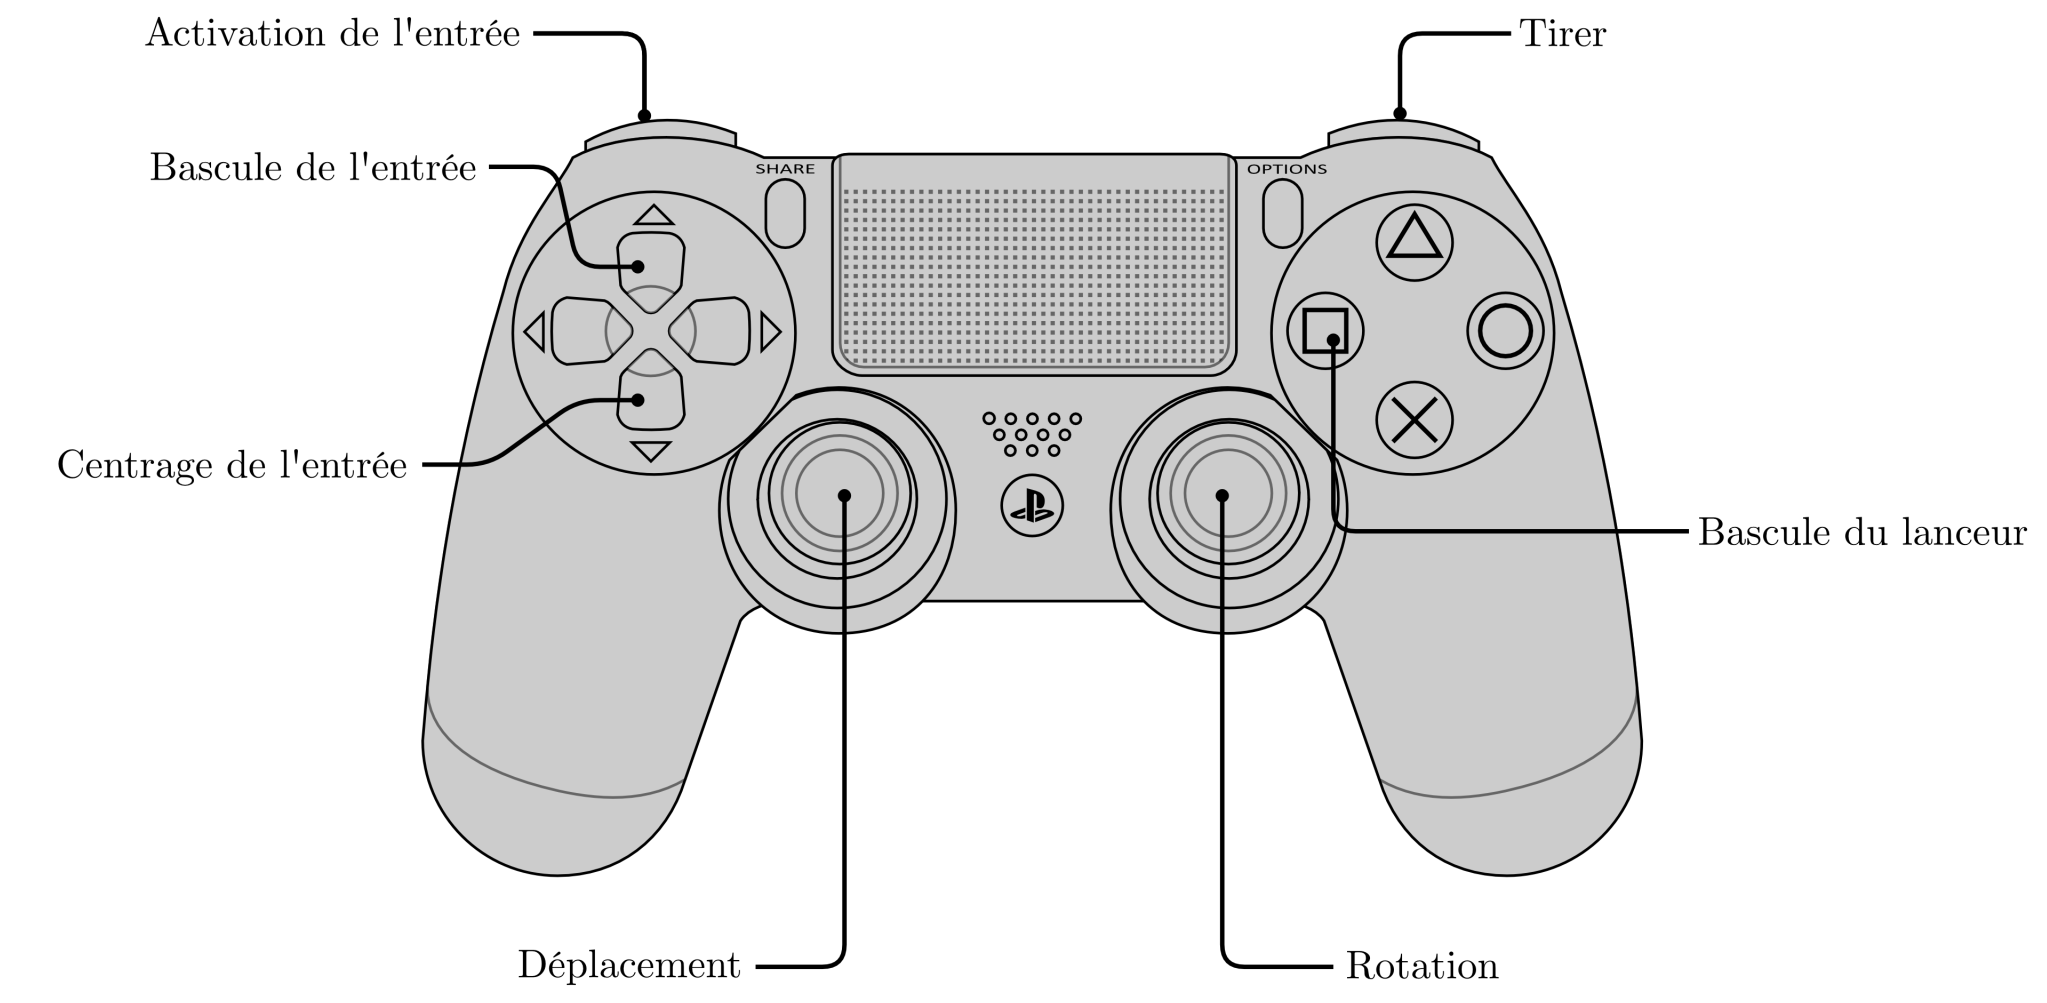
\includegraphics[width=\textwidth,inkscapelatex=true]{GAMEPAD-DIAGRAM.pdf}
    \caption{Schéma des commandes du gamepad}
    \label{fig:gamepad-diagram}
\end{figure}

\needspace{10\baselineskip}
\subsubsection{Déplacement du robot}

Le robot utilise un châssis à roues omnidirectionnelles, permettant des déplacements dans toutes les directions.

\begin{itemize}
    \item Utilisez le joystick gauche pour contrôler la translation (avant/arrière et gauche/droite).
    \item Utilisez le joystick droit pour contrôler la rotation du robot (droite/gauche).
    \item Ralentissez la vitesse de déplacement ou de rotation en cliquant sur les joysticks.
\end{itemize}

\begin{myinfo}{Modes de déplacement}
    Le robot peut se déplacer en plusieurs modes:
    \begin{itemize}
        \item \textbf{Field-centric :} Le robot se déplace en fonction du terrain, indépendamment de son orientation.
        \item \textbf{Robot-centric :} Le robot se déplace en fonction de son orientation actuelle.
    \end{itemize}
    Par défaut, le mode field-centric est activé pour une meilleure intuitivité.
    Il est possible d'utiliser le mode robot-centric, cependant il faut désactiver le suivi de pose qui empêche de nombreuses fonctionnalités.
\end{myinfo}

\subsubsection{Entrée}

Le robot est équipé d'un système d'entrée pour ramasser les \textit{artifacts}.
\begin{itemize}
    \item Appuyez sur le bouton \texttt{L2} pour activer l'intake et ramasser les \textit{artifacts}. Une fois le bouton relâché, l'intake s'arrête.
    \item Appuyez sur le bouton \texttt{$\downarrow$} pour centrer l'intake switcher, permettant de ramasser plus rapidement les \textit{artifacts}.
    \item Appuyez sur le bouton \texttt{$\uparrow$} pour basculer l'intake switcher, permettant de forcer le ramassage d'un côté spécifique.
\end{itemize}

\begin{myinfo}{Attention!}
    Il est très important de faire rentrer les \textit{artifacts} en alternant les côtés, afin d'éviter les blocages et les erreurs de sélection.
    Par exemple, si le dernier \textit{artifact} a été ramassé à gauche, le suivant doit être ramassé à droite.

    Si deux \textit{artifacts} sont ramassés du même côté, le robot ne pourra pas prendre le troisième. Il risque aussi de pousser les artifacts dans le lanceur, le bloquant ou causant des erreurs de tir.
\end{myinfo}

\subsubsection{Tirer}

Le robot est équipé d'un lanceur à flywheel pour tirer les \textit{artifacts} dans le but.

\begin{itemize}
    \item Appuyez sur le bouton \textttt{$\square$} pour préparer le tir. La flywheel accélérera à la vitesse cible. Appuyez à nouveau sur le bouton pour arrêter la flywheel.
    \item Une fois la vitesse atteinte, appuyez sur le bouton \texttt{R2} pour tirer l'\textit{artifact}. Le buffer poussera l'\textit{artifact} dans le lanceur.
\end{itemize}

Si le robot détecte que le driver essaie de tirer sans que la flywheel soit à la bonne vitesse, il n'autorisera pas le tir et fera vibrer le gamepad pour avertir le pilote.

\section{Scénarios de match}

\begin{myinfo}{Manque de données}
    Cette section est incomplète à cause d'un manque de données lié au faible nombre de tests et de matchs réalisées.
\end{myinfo}

\section{Séquences autonomes}
\section{Gestion des erreurs et dépannage}

\end{document}